\documentclass[aspectratio=169]{beamer}

% ---------- Theme ----------
\usetheme{Madrid}
\usecolortheme{default}
\usepackage{xcolor}

% Define maroon
\definecolor{maroon}{RGB}{128,0,0}

% Apply to theme
\setbeamercolor{structure}{fg=maroon}
\setbeamercolor{frametitle}{fg=white, bg=maroon}
\setbeamercolor{block title}{bg=maroon, fg=white}
\setbeamercolor{block body}{bg=maroon!8, fg=black}
\setbeamercolor{item}{fg=maroon}
\setbeamercolor{title}{fg=white}
\setbeamercolor{subtitle}{fg=maroon!85!black}
\setbeamercolor{author}{fg=black}
\setbeamercolor{date}{fg=black}
\setbeamercolor{institute}{fg=black}

% ---------- Packages ----------
\usepackage{graphicx}
\usepackage{booktabs}
\usepackage{amsmath, amssymb}
\usepackage{hyperref}
\usepackage{listings}
\usepackage{tikz}
\usetikzlibrary{arrows.meta,positioning}

% ---------- Listings (code) ----------
\lstset{
  basicstyle=\ttfamily\small,
  breaklines=true,
  frame=single,
  showstringspaces=false
}

% ---------- Meta ----------
\title{Kalshi Market Making Algorithm}
\author{George Lord, Chris Mulligan, and Max Zhalilo \\ (12243747, 12502987, 12341701)}
\date{\today}

\begin{document}

% ---------- Title slide ----------
\begin{frame}[plain]
  \titlepage
\end{frame}

% ---------- Agenda ----------
\begin{frame}{Agenda}
  \begin{enumerate}
    \item Overview
    \item Kalshi SPX Event Contracts
    \item Replication by Binary Calls/Puts
    \item Modeling SPX Price CDF Log-Normally
    \item Kalshi Market Making from Fair Prices (VIX-based Spread)
    \item Delta-Hedging Kalshi Contracts with SPY
    \item Steps Together
    \item Required Data and Computations
  \end{enumerate}
\end{frame}

% ---------- Section ----------
\section{Overview}

\begin{frame}{Overview}
  \begin{itemize}
    \item We run automated market-making strategies on short-term (0-1 Day) SPX Price Events.
    \item We model the probability of SPX being above/below a price at a given time log-normally, using live SPX and VIX.
    \item We use this to fair price binary calls/puts, then fair price Kalshi SPX events via replication.
    \item We also use VIX to adjust position sizing.
    \item We hedge our delta exposure with SPY.
  \end{itemize}
\end{frame}

% ---------- Figure slide ----------
\begin{frame}{Kalshi Contract 1: KXINXU}
\begin{columns}[T,onlytextwidth]
  % Left: image
  \begin{column}{0.48\textwidth}
    \centering
    \includegraphics[width=\linewidth]{KXINXU.png}
    \vspace{0.2em}
    \scriptsize The KXINXU market for Feb 26, 2026, which has resolved
  \end{column}

  % Right: bullet points
  \begin{column}{0.52\textwidth}
    \small
    \begin{itemize}
      \item KXINXU (as prefixed by Kalshi API) contracts bet whether the end-of-day S\&P 500 index value will be above a given value after a specific day and time in the future (as measured by SPX value)
      \item "Yes" and "No" contracts at various index values are actively traded 24/7 leading up to the last trading day, after which contracts are paid out. Each contract for a correct prediction pays out \$1, and wrong predictions pay out \$0
      \item As such, "Yes" contracts act as binary calls on SPX, and "No" contracts as binary puts, for a given strike price (the "above" price, e.g. \$6,875) and expiration date (2/26/26 4PM EST in this example)
    \end{itemize}
  \end{column}
\end{columns}
\end{frame}

% ---------- Figure slide ----------
\begin{frame}{Kalshi Contract 2: KXINX}
\begin{columns}[T,onlytextwidth]
  % Left: image
  \begin{column}{0.48\textwidth}
    \centering
    \includegraphics[width=\linewidth]{KXINX.png}
    \vspace{0.2em}
    \scriptsize The KXINX market for Feb 26, 2026, which has resolved
  \end{column}

  % Right: bullet points
  \begin{column}{0.52\textwidth}
    \small
    \begin{itemize}
      \item KXINX contracts bet whether the end-of-day S\&P 500 index value will fall in a specific range after a specific day and time in the future (as measured by SPX value)
      \item "Yes" contracts can be replicated as a position long one binary call with strike at the bottom of the range, and short one binary call with strike at the bottom of the range (binary call spread). "No" contracts would be replicated by going long one binary put at the bottom of the range, and long one binary call at the top of the range (binary strangle).
    \end{itemize}
  \end{column}
\end{columns}
\end{frame}

\begin{frame}{Binary Call/Put Risk-Neutral Pricing}
  Recall that a binary call on $S$ expiring at time $T$ with strike $K$ has risk-neutral time $t < T$ price of:
  \[
    V_t = e^{-\int_t^Tr(u)du}\mathbb{Q}_t(S_T > K)
  \]
  where
  \begin{itemize}
    \item $e^{-\int_t^Tr(u)du}$ is the discount factor based on risk-free rate $r$
    \item $\mathbb{Q}_t(S_T > K)$ is the risk-neutral probability of $S$ finishing over $K$ at time $T$ \newline(based on all info at time $t$)
  \end{itemize}

Similarly, a binary call has a risk-neutral price equal to the discounted risk-neutral probability of $S$ finishing under $K$ at time $T$.
\end{frame}

\section{Replication}

\begin{frame}{Replication}
  \begin{block}{Key Observation}
    All of these Kalshi contracts can be replicated with (combinations of) binary calls/puts
  \end{block}

  \begin{alertblock}{Implications}
    \begin{itemize}
      \item At 0 to 1 DTE, binary call/put prices approach the probability of SPX ending above/below a given price (discount $\to$ $1$ as $T-t \to 0$)
      \item If we know/can accurately estimate these probabilities, we can fairly price binary calls/puts on SPX, and therefore (via replication) fairly price KXINXU and KXINX for a given SPX price/range and expiration
    \end{itemize}
  \end{alertblock}
\end{frame}

\begin{frame}{Modeling SPX Price CDF Log-Normally}
  Remaining consistent with the typical Black-Scholes (lognormal) model for binary calls/puts, we can model the required probabilities as:
  \[
    \mathbb{P}_t(S_T > K) = \Phi(d_2(K)) \text{ and } \mathbb{P}_t(S_T < K) = 1 - \mathbb{P}_t(S_T > K)
  \]
  
  \[
    d_2(K) = \frac{\ln{(F/K)} - \frac{1}{2}\sigma^2(T-t)}{\sigma\sqrt{T-t}}
  \]
  
  where
  \begin{itemize}
    \item $F \approx S_t = $ current SPX value (since discount is negligible with 0 to 1 DTE, don't trade over dividends)
    \item $K$ is the corresponding binary strike price
    \item $T$ is the corresponding contract resolution date+time, and $t$ the current time, such that $T - t$ is in years (float64)
    \item $\sigma$ is assumed flat and taken from current VIX in percent $ / 100$
  \end{itemize}

\end{frame}

\begin{frame}{Scaling Market-Making Bid-Ask Spread with VIX}
  In market making, our position size is directly related to the spread width at which we bid/ask. We have fair values for Kalshi contracts for a given price (range) and time to expiration. We can use this as the center for each contract, and then adjust our width based on VIX. We will test various methods for this as part of our project, but they will generally:
 
  \begin{itemize}
    \item Use our fair-prices for the contracts as described before as our center
    \item Calculate our bid-ask spread width as a function of
        \begin{itemize}
            \item Real-time VIX level (as a measure of volatility)
            \item Time to Kalshi Expiration (e.g. time to 2/26/26 4PM EST in prev. examples)
            \item Our current net position in YES shares (positive = long YES)
            \item Tick size (usually 1 cent)
            \item Kalshi's fees (so we don't post bid/asks with -EV after fees)
        \end{itemize}
    \item We will generally widen as settlement approaches and volatility rises.
  \end{itemize}

\end{frame}

\begin{frame}{Delta-Hedging with SPY}
  In order to remove directional risk from SPX moves as we accumulate Kalshi positions by market-making (and being filled), we will delta-hedge with SPY. Because our Kalshi contract fair values are a function of current SPX, and since the SPY ETF has (by construction) a delta $\frac{\partial\text{SPY}}{\partial\delta{\text{SPX}}} \approx \frac{\text{SPY}}{\delta{\text{SPX}}} \approx 0.1$, we can delta hedge a Kalshi contract by calculating the net delta of it's replication's individual binary call/puts via:
  \[
    \Delta_{\text{YES ABOVE}}(K) = \frac{\partial(\Phi(d_2(S)))}{\partial S} = \frac{\varphi(d_2(S_t))}{S_t\sigma\sqrt{T-t}} \text{ and } \Delta_{\text{NO ABOVE}}(K) = -\Delta_{\text{YES ABOVE}}(K)
  \]

then summing all our open Kalshi position deltas $\Delta_i$ by their quantity $q_i$ as:

  \[
    \Delta_{\text{book,SPX}} = \sum_i q_i\Delta_i
  \]

which is in dollars of contact value per 1 SPX point. Since $10$ SPX point $\approx$ $1$ SPY dollars, we take position
\[
    -10\Delta_{\text{book,SPX}} \text{ shares of SPY}
\]

\end{frame}


\begin{frame}[c]{Putting it Together}
\centering

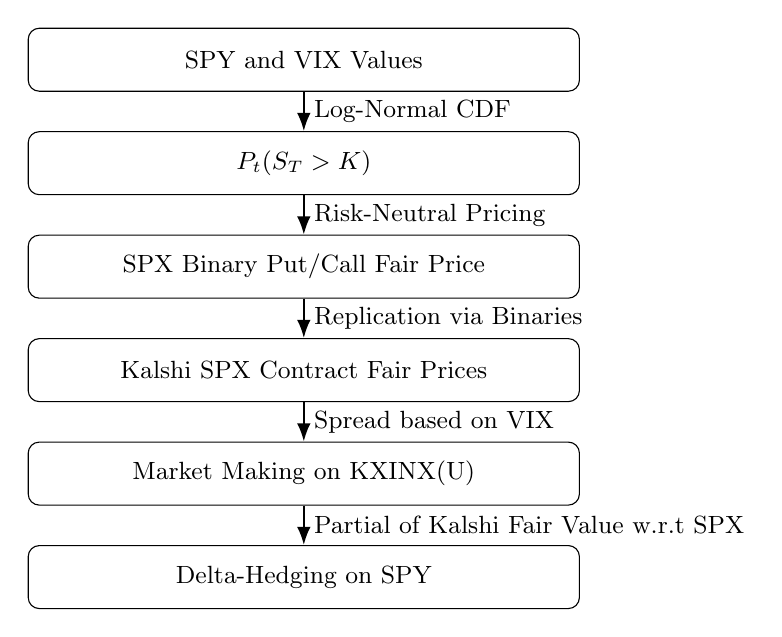
\begin{tikzpicture}[
    font=\small,
    node distance=5mm,
    box/.style={draw, rounded corners, align=center, minimum width=70mm, minimum height=8mm},
    arrow/.style={-Latex, thick}
]
\node[box] (a) {SPY and VIX Values};
\node[box, below=of a] (b) {$P_t(S_T > K)$};
\node[box, below=of b] (c) {SPX Binary Put/Call Fair Price};
\node[box, below=of c] (d) {Kalshi SPX Contract Fair Prices};
\node[box, below=of d] (e) {Market Making on KXINX(U)};
\node[box, below=of e] (f) {Delta-Hedging on SPY};

\draw[arrow] (a) -- node[right]{Log-Normal CDF} (b);
\draw[arrow] (b) -- node[right]{Risk-Neutral Pricing} (c);
\draw[arrow] (c) -- node[right]{Replication via Binaries} (d);
\draw[arrow] (d) -- node[right]{Spread based on VIX} (e);
\draw[arrow] (e) -- node[right]{Partial of Kalshi Fair Value w.r.t SPX} (f);
\end{tikzpicture}

\end{frame}



% --- Data ---

\begin{frame}{Required Data and Computations}
  \begin{columns}[T,onlytextwidth]
    \begin{column}{0.52\textwidth}
      \textbf{(Historical) Data Sources}
      \begin{itemize}
        \item 1s OHLCV SPY from Databento
        \item 1s SPX and VIX values from Bloomberg
        \item KXINX(U) Contract specs (settlement, "strike" prices, ranges) from Kalshi API
        \item KXINX(U) Order book updates from Kalshi API
        \item (Possibly) risk-free rate data for discounting (e.g. SOFR OIS)
      \end{itemize}
    \end{column}
    \begin{column}{0.48\textwidth}
      \textbf{Computations}
      \begin{itemize}
        \item SPX CDF over historical time-series
        \item Implied KXINXU binary call/put fair values
        \item Implied KXINX binary combo fair values
        \item Our KXINX(U) bid/asks based on fair values, VIX, and Kalshi historical data
        \item Simulated fills based on Kalshi historical and assumed $p_\text{fill}$
        \item Deltas and delta-hedges based on simulated fills, SPY historical, and fair value partials
        \item Trades, PnL, and performance metrics based on simulated fills and SPY hedges
      \end{itemize}
    \end{column}
  \end{columns}
\end{frame}


\end{document}